%
%  untitled
%
%  Created by Martin Mroz on 2009-02-03.
%  Copyright (c) 2009 __MyCompanyName__. All rights reserved.
%
\documentclass[]{article}

% Use utf-8 encoding for foreign characters
\usepackage[utf8]{inputenc}

% Setup for fullpage use
\usepackage{fullpage}

% Uncomment some of the following if you use the features
%
% Running Headers and footers
%\usepackage{fancyhdr}

% Multipart figures
%\usepackage{subfigure}

% More symbols
%\usepackage{amsmath}
%\usepackage{amssymb}
%\usepackage{latexsym}

% Surround parts of graphics with box
\usepackage{boxedminipage}
\usepackage{multicol}

% Package for including code in the document
\usepackage{listings}

% If you want to generate a toc for each chapter (use with book)
\usepackage{minitoc}

% This is now the recommended way for checking for PDFLaTeX:
\usepackage{ifpdf}

%\newif\ifpdf
%\ifx\pdfoutput\undefined
%\pdffalse % we are not running PDFLaTeX
%\else
%\pdfoutput=1 % we are running PDFLaTeX
%\pdftrue
%\fi

\setlength{\parindent}{0pt} 
\setlength{\parskip}{2ex}

\ifpdf
\usepackage[pdftex]{graphicx}
\else
\usepackage{graphicx}
\fi

\lstset{
  basicstyle=\small,
  keywordstyle=\bfseries,
  identifierstyle=,
  commentstyle=\slshape,
  stringstyle=\ttfamily,
  showstringspaces=false
  frame=leftline,
  numbers=left,
  numberstyle=\tiny,
  stepnumber=1,
  numbersep=-4pt
}

\newcommand{\ModLang}{LQX }
\newcommand{\lqns}{Layer Queueing Network Solver}

\begin{document}

  \ifpdf
  \DeclareGraphicsExtensions{.pdf, .jpg, .tif}
  \else
  \DeclareGraphicsExtensions{.eps, .jpg}
  \fi
  
  % -------------------------------------------------------- [Title Page]
  
  \vskip 1.0in
  \pagestyle{empty}
  {\LARGE \textbf{\ModLang Programmers Guide}}\\
  {\large General Purpose Language for Simulation Modeling}\\
  {\small Wednesday, 13 May 2009 - Martin Mroz}
  \newpage
  
  % -------------------------------------------------------- [Table of Contents]
  
  \pagestyle{plain}
  \tableofcontents
  \newpage
  
  % -------------------------------------------------------- [Introduction]
  
  \section{Programmers' Overview of \ModLang}
  
  In keeping with the design intentions, \ModLang is an extremely simple
  programming language interpreter/compiler hybrid. The initial incarnation of
  the full self-contained \ModLang library weighs in at little over 4000 lines. The
  library is written in plain C++ with collections provided by the STL. Making 
  modifications or extensions to either the grammar of the language or the
  built-in APIs is extremely simple, and the changes have limited scope. The
  purpose of this document is to lay out the architecture of the \ModLang library
  for primarily for programmers wishing to either modify the grammar or to add
  new APIs or Objects (either built into the \ModLang library or for applications
  wishing to make use of \ModLang).
  
  \newpage
  % -------------------------------------------------------- [Basic Architecture]
  
  \section{\ModLang Client Applications}
  \subsection{Procedure for Invoking \ModLang Programs}
  
  Since these programs are likely to only be run once and be relatively uncomplicated, 
  the benefits of substantial compile-time optimizations such as IR/bytecode generation 
  are outweighed by their costs. The following flowchart illustrates how incoming LQX
  code is compiled into a {\tt Program} instance which can then be invoked by client
  applications (such as LQNS2).
  
  \begin{figure}[htbp]
    \centering
      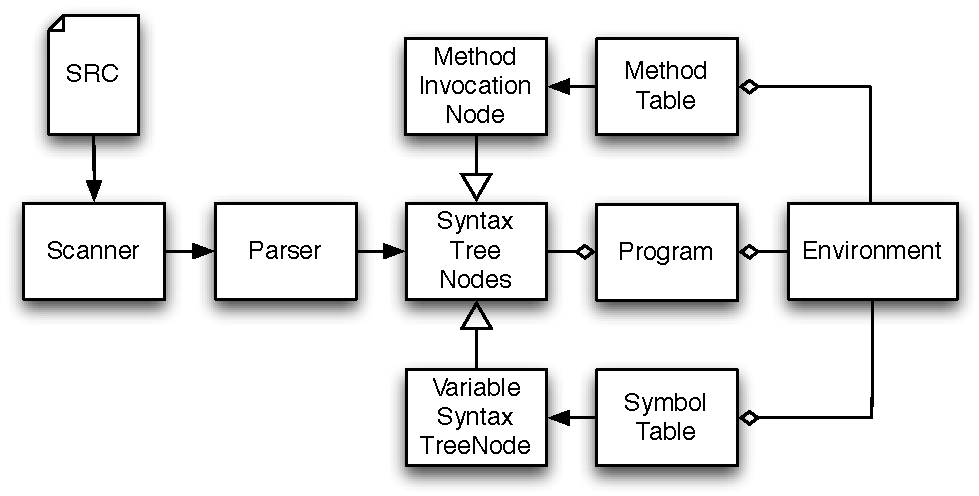
\includegraphics[scale=0.7]{flowchart.pdf}
    \caption{Data Flow and Ownership Map for the LQX Runtime}
    \label{fig:flowchart}
  \end{figure}
  
  The majority of the external API for the \ModLang system is exposed in five class groups:
  {\tt Program}, {\tt Environment}, {\tt Method/MethodTable}, {\tt Symbol/SymbolTable} 
  and {\tt LanguageObject}. In general, taking a piece of \ModLang code from plain text to
  running and then to post-cleanup involves the following:
  
  \begin{enumerate}
    \item Your application invokes {\tt Program::loadFromText()}.
    \item The LQX source file is scanned and parsed to create a {\tt Program} instance.
    \item You configure the {\tt Environment} by some combination of:
      \begin{enumerate}
        \item Defining and setting up External Variables in the Symbol Table.
        \item Registering Methods in the Method Table.
      \end{enumerate}
    \item Calling {\tt Program.invoke()}
    \item Destroying the {\tt Program} instance.
  \end{enumerate}
  
  The LQX runtime by itself exposes a small but powerful set of basic APIs so that users
  will have a consistent experience with \ModLang code regardless of the client application.
  These APIs are documented in the \ModLang Users' Manual document, but include for example
  basic Array creation, manipulation and traversal and floating-point operations that
  are not expressed within the grammar. Thus, in order for \ModLang to provide the user
  the ability to interact with your program, you will have to provide so-called 
  ``Bindings'' for \ModLang. This can consist of a set of global methods by themselves
  or in combination with ``Language Objects.'' The following sections cover how one would
  go about completing items 3a and 3b from the list above, that is the creation and 
  registration of language bindings for your \ModLang client program.
  
  \subsection{Defining Bindings using Global Methods}
  
  In \ModLang, global methods are functions which users can freely invoke within their source
  code. When they do so, it will trigger the invocation of a method within the client application.
  Even Methods in the \ModLang language are actually instances of classes. This cleans up and
  simplifies their handling internally within the \ModLang runtime. This means that for the
  client application to define their own methods requires them to subclass the {\tt Method} type.
  The only way to create instances of Language Objects, described in the subsequent section, is
  by the invocation of a global method.
  
  To make it easier for developers to limit the argument types which are passed into a method
  invocation (due to the loose typing), a ``string'' of characters which indicate a certain
  restrictions on the argument types. The different values are as follows:
  
  \begin{description}
    \item[\ \ \ \ b] A boolean argument must be provided.
    \item[\ \ \ \ d] A numeric argument must be provided.
    \item[\ \ \ \ s] A string argument must be provided.
    \item[\ \ \ \ o] An object instance argument must be provided.
    \item[\ \ \ \ a] This argument can be any type (b-, d-, s- or o-type).
    \item[\ \ \ \ 1] This must be at the end of the string. Allows either 0 or 1 argument of any type.
    \item[\ \ \ \ +] This must be at the end of the string. Allows any number (0 to n) more of any type.
  \end{description} 
  
  For example, a method which can take 2 numeric arguments would use the string ``dd'', the
  {\tt print} method uses the string ``+'' and the {\tt floor} method uses the string ``d''.
  
  The following code listing defines the {\tt super\_sum(numeric n1, numeric n2)} language method.
  When the runtime encounters a call of this method, it will resolve all of the arguments down
  to their {\tt Symbol} values and pass them into {\tt Method.invoke(Environment* env,
  std::vector<SymbolAutoRef>\& args)}. The class declaration would be as follows:
  
  \lstset{language=C++}
  \begin{lstlisting}
  class SuperSumMethod : public Method {
  public:
    virtual std::string getName() const { return "super_sum"; } 
    virtual const char* getParameterInfo() const { return "dd"; } 
    virtual std::string getHelp() const { return "Returns 3*arg1 + arg2"; }
    virtual SymbolAutoRef invoke(Environment* env, 
      std::vector<SymbolAutoRef >& args) throw (RuntimeException);
  };
  \end{lstlisting}
  
  For programmer convenience, this can be written shorthand using the macro 
  {\tt DeclareLanguageMethod (class\_name, param\_str, func\_name, help)} which will evaluate to
  exactly what is shown in the listing above. Similarly, the actual implementation can
  either be written out in its entirety or by using {\tt InplementLanguageMethod (class\_name)}.
  
  \lstset{language=C++}
  \begin{lstlisting}
  SymbolAutoRef SuperSumMethod::invoke(Environment* env, 
    std::vector<SymbolAutoRef >& args) throw (RuntimeException) {
    double arg1 = decodeDouble(args, 0);
    double arg2 = decodeDouble(args, 2);
    double result = (3 * arg1) + arg2;
    return Symbol::encodeDouble(result);
  }
  \end{lstlisting}
  
  So once you have finished declaring and implementing your global methods, you must go
  ahead and register them with the {\tt Environment}. When you call this method is up to you,
  but it depends on the {\tt Environment} instance for a given {\tt Program} instance, so
  it must be done after a program has been successfully loaded.
  
  \lstset{language=C++}
  \begin{lstlisting}
  Environment* env = program->getEnvironment();
  MethodTable* mt = env->getMethodTable();
  mt->registerMethod(new SuperSumMethod());
  \end{lstlisting}
  
  Thus, we can go ahead an invoke our new method as shown in the following \ModLang snippet:
  
  \lstset{language=C++}
  \begin{lstlisting}
  m1 = 9.0;
  m2 = 12.0;
  r = super_sum(m1, m2);
  print("3 * ", m1, " + ", m2, " = ", r);
  \end{lstlisting}
  
  \subsection{Defining Bindings Using Objects}
  
  The \ModLang client API allows the definition of semi-opaque ``Language Objects.'' An example
  of a Language Object would be the {\tt Array} object built-in type. With Language Objects,
  you can define a set of attributes which can be exposed via the language directly or define
  a set of global methods which take the object as one of their arguments, customarily the first.
  Examples of such methods include {\tt array\_get(object array, ? key)} and 
  {\tt array\_has(object array, ? key)}.
  
  As with a method, a Language Object is also an object within the scope of the runtime. It
  must be a subclass of the {\tt LanguageObject} type. Doing so allows the runtime to take care
  of lifecycle management automatically. Each custom object must implement a certain core
  set of methods that allow it to coexist with all others, such as some comparison 
  operators ({\tt operator=()} and {\tt operator<()}), some name and description methods.
  These allow user-defined objects to participate as {\tt Array} keys, amongst other things.
  The following listing implements a {\tt ColorObject} class which stores a color value
  as 4 components (RGBA), and implements all the recommended methods. This particular class 
  exposes 4 properties to the language {\tt r}, {\tt g}, {\tt b} and {\tt a},
  the four components of the color. 
  
  \lstset{language=C++}
  \begin{lstlisting}
  #include <sstream>
  #include "lqx/LanguageObject.h"
  class ColorObject : public LanguageObject {
  public:

    /* The Unregistered Type ID for Colors is 100+0 */
    static const uint32_t kColorObjectTypeId = 100+0;

  public:

    /* Class Structors */
    ColorObject(double r, double g, double b, double a) : 
      LanguageObject(kColorObjectTypeId),
      _r(r), _g(g), _b(b), _a(a) {}
    virtual ~ColorObject() {}

    /* Optional overrides for testing */
    virtual bool isEqualTo(LanguageObject* other)
    {
      /* Make sure that the type Ids match up right*/
      if (getTypeId() != other->getTypeId()) {
        return false;
      }

      /* Compares all of the different bits */
      ColorObject* co = (ColorObject *)other;
      return (_r == co->_r) && (_g == co->_g) &&
        (_b == co->_b) && (_a == co->_a);
    }

    virtual bool isLessThan(LanguageObject* other)
    {
      /* Make sure that the type Ids match up right*/
      if (getTypeId() != other->getTypeId()) {
        return this->LanguageObject::isLessThan(other);
      }

      /* Make sure that (1,0,0,0) is not equal to (0,0,0,1) */
      ColorObject* co = (ColorObject *)other;
      double total = (1000 * _r) + (100 * _g) + (10 * _b) + _a;
      double ototl = (1000 * co->_r) + (100 * co->_g)
       + (10 * co->_b) + co->_a;
      return total < ototl;
    }

    virtual std::string description()
    {
      /* Description for str() and print() */
      std::stringstream ss;
      ss << "(r=" << _r << ",g=" << _g <<
        ",b=" << _b << ",a=" << _a << ")";
      return ss.str();
    }

    virtual std::string getTypeName()
    {
      /* Human-readable type name */
      return "Color";
    }

    virtual SymbolAutoRef getPropertyNamed(Environment* env, 
      std::string name) throw (RuntimeException)
    {
      /* We have r,g,b and a as properties */
      if (name == "r") {
        return Symbol::encodeDouble(_r);
      } else if (name == "g") {
        return Symbol::encodeDouble(_g);
      } else if (name == "b") {
        return Symbol::encodeDouble(_b);
      } else if (name == "a") {
        return Symbol::encodeDouble(_a);
      }

      /* Call up to the superclass for the LanguageObject properties */
      return this->LanguageObject::getPropertyNamed(env, name);
    }

  private:

    /* Actual storage of the values */
    double _r, _g, _b, _a;

  };
  \end{lstlisting}
  
  Now we have an object which the language can make use of and manage for us, but
  we don't have any way of creating them. For this, we need to define a Global Language
  Method. In our case we call it, by convention, {\tt color\_create (numeric r,
  numeric g, numeric b, numeric a)} which returns a new instance of ColorObject. This
  is accomplished using short-hand notation as follows:
  
  \lstset{language=C++}
  \begin{lstlisting}
  static inline double clamp(const double input) {
    double c = (input < 0) ? 0 : input;
    c = (c > 1) ? 1 : c;
    return c;
  }
  
  DeclareLanguageMethod (color_create, "dddd", "color_new", 
    "Creates an instance of Color.");
  ImplementLanguageMethod (color_create) {
    double r = clamp(decodeDouble(args, 0));
    double g = clamp(decodeDouble(args, 1));
    double b = clamp(decodeDouble(args, 2));
    double a = clamp(decodeDouble(args, 3));
    return Symbol::encodeObject(new ColorObject(r,g,b,a), false);
  }
  \end{lstlisting}
  
  Thus we have effectively linked the \ModLang runtime to the native code within
  your program, and allowed users to access it at will. In implementing language methods,
  the only level of granularity checked by the runtime is that a given parameter is an
  object where specified, but not which kind. This must be done by the callee, as shown
  in {\tt ColorObject.isEqualTo()}, as a ``safe'' cast. Bringing everything together,
  we can now execute the following \ModLang program:
  
  \lstset{language=C++}
  \begin{lstlisting}
  c = color_new(0.2, 0.4, 0.6, 0.8);
  print("Color description is ", c);
  print("red = ", c.r, " green = ", c.g, " blue = ", c.b, " alpha = ", c.a);
  \end{lstlisting}
  
  \subsection{Binding External Variables}
  
  In certain cases, a program will want to have some variables shared between the
  \ModLang runtime and the application itself. This is accomplished using what are known
  as ``External Variables.'' In order to obtain one, once a program is loaded and 
  before it is run you must simply invoke {\tt Program.getExternalVariable()}. If 
  you want it to be modifiable from within the program you simply call
  {\tt SymbolAutoRef.setIsConstant(false)}. It will be constant by default.
  This will save a lot of code by eliminating the need for APIs for setting
  values in the program from the \ModLang program.
  
  % ------------------------------------------------------------------------------------------
  
  \section{Changing the LQX Runtime or Interpreter}
  \subsection{General Overview of Architecture}
  
  As mentioned earlier in the text, the LQX runtime/interpreter was designed to compile code
  as quickly as possible, and to run it reasonably fast. As such, the approach taken was that
  or a hybrid interpreter/compiler. Rather than compiling to bytecode directly or even into
  an intermediate representation, compilation stops at the syntax tree phase. Each syntax tree
  node comes equipped with two methods:
  
  \ \ \ \ {\tt virtual void debugPrintGraphviz(std::stringstream\& output); }\\
  \null\ \ \ \ {\tt virtual SymbolAutoRef invoke(Environment* env) throw (RuntimeException);}
  
  Thus it becomes possible to either print a GraphViz representation of the syntax tree from
  this point down for debugging purposes or to directly invoke the syntax tree node with the
  expectation of receiving a {\tt SymbolAutoRef} (NULL or not) from it. 
  
  The idea is that the program text is loaded into memory, scanned by the {\tt Scanner}, 
  converted into a series of {\tt SyntaxTreeNode} instances by the {\tt Parser}, which
  then wraps them in an instance of {\tt Program}. This program, when executed, invokes
  all root level {\tt SyntaxTreeNode} instances which form the flow of control of the program.
  It is the appropriate {\tt SyntaxTreeNode}s which actually interact with either the
  {\tt MethodTable} or the {\tt SymbolTable}. This flow is best illustrated in 
  Figure~\ref{fig:flowchart}.
  
  \newpage
  % ------------------------------------------------------------------------------------------
  
  \section{The LQX Language BNF}
  
  \lstset{language=C++}
  \begin{lstlisting}
  <program>          ::= <stmt_list>
  <stmt_list>        ::= <stmt> | <stmt_list> <stmt>
  <stmt>             ::= <expr_stmt> | <conditional_stmt> 
                       | <compound_stmt> | <loop_stmt>
  <compound_stmt>    ::= "{" "}" | "{" <stmt_list> "}"
  
  <loop_stmt>        ::= "while" "(" <expr> ")" <stmt>
                       | "foreach" "(" <ID> "," <ID> "in" <expr> ")" <stmt>
                       | "foreach" "(" <ID> "in" <expr> ")" <stmt>
                       | "for" "(" <expr_stmt> <expr_stmt> <opt_e> ")" <stmt>
  <opt_e>            ::= . | <expr>
  
  <conditional_stmt> ::= "if" "(" <expr> ")" <stmt> <opt_else>
  <opt_else>         ::= . | "else" <stmt>
  
  <expr_stmt>        ::= ";" | <expr> ";"
  <expr>             ::= <assignment_stmt> | <expr> "," <assignment_stmt>
  <assignment_stmt>  ::= <logic_or_stmt> | <assignment_stmt> "=" <logic_or_stmt>
  <logic_or_stmt>    ::= <logic_and_stmt> | <logic_or_stmt> "||" <logic_and_stmt>
  <logic_and_stmt>   ::= <relation_stmt> | <logic_and_stmt> "&&" <relation_stmt>
  <relation_stmt>    ::= <compare_stmt> 
                       | <relation_stmt> "==" <compare_stmt>
                       | <relation_stmt> "!=" <compare_stmt>
  <compare_stmt>     ::= <shift_stmt>
                       | <compare_stmt> "<" <shift_stmt>
                       | <compare_stmt> "<=" <shift_stmt>
                       | <compare_stmt> ">" <shift_stmt>
                       | <compare_stmt> ">=" <shift_stmt>
  <shift_stmt>       ::= <add_sub_stmt>
                       | <shift_stmt> ">>" <add_sub_stmt>
                       | <shift_stmt> "<<" <add_sub_stmt>
  <add_sub_stmt>     ::= <mul_div_stmt>
                       | <add_sub_stmt> "+" <mul_div_stmt>
                       | <add_sub_stmt> "-" <mul_div_stmt>                    
  <mul_div_stmt>     ::= <prefix_stmt>
                       | <mul_div_stmt> "*" <prefix_stmt>
                       | <mul_div_stmt> "/" <prefix_stmt>
                       | <mul_div_stmt> "%" <prefix_stmt>
  <prefix_stmt>      ::= <vpf_stmt> | "!" <vpf_stmt>
  <vpf_stmt>         ::= <postfix_stmt>
                       | <vpf_stmt> "[" <logic_or_stmt> "]"
                       | <vpf_stmt> "." <ID>
  <postfix_stmt>     ::= <basic_stmt>
                       | <ID> "(" ")"
                       | <ID> "(" <expr_list> ")"
  <basic_stmt>       ::= <NULL> | <STRING> | <DOUBLE> | <BOOLEAN> | <ID>
                       | "[" <expr_list> "]" | "[" "]" 
                       | "{" <map_list> "}" 
                       | "(" <expr> ")"
  
  <expr_list>        ::= <assignment_stmt> | <expr_list> "," <assignment_stmt>
  <map_list>         ::= <assignment_stmt> "=>" <assignment_stmt>
                       | <map_list> "," <assignment_stmt> "=>" <assignment_stmt> 
  \end{lstlisting}
  
\end{document}
